\chapter{\xlabel{fcfsred}FCFs by Reduction Date}
\label{app:fcfs}

Ongoing development of the SCUBA-2 analysis has resulted in ongoing
changes to the atmospheric opacity relationships and the FCFs.
Depending on when your data were reduced you will need to apply
different calibration values. \textsc{orac-dr} will automatically apply
the appropriate values.

\textbf{Note:} As of the 2021A Starlink release, the
opacity relations and FCF values have been updated following the
results presented by Mairs et al. 2021 \cite{mairs21}. Historical values derived by Dempsey et al. 2013
\cite{dempsey12} are presented below the updated values for comparison.

\vspace{1cm}

\textbf{Explanation of parameters} (see also \cref{Appendix}{app:cal}{SCUBA-2 data calibration}):

Starlink currently applies the following multiplicative extinction correction to SCUBA-2 data:

\begin{equation}
\mathrm{Extinction\:Correction} = \frac{1}{\mathrm{exp}[-\tau_{\nu}\times\mathrm{Airmass}]}
\end{equation}
where $\tau_{\nu}$ is the atmospheric opacity at the given frequency, $\nu$. ``Opacity relations''
relate the measured $\tau_{225}$ to the atmospheric opacity at the operating frequencies of
SCUBA-2, $\tau_{666}$ (450~$\mu$m) and $\tau_{345}$ (850~$\mu$m). Their form is:
\begin{equation}
\label{eq:2021taurelation}
\tau_{\nu} = \mathrm{a}\times(\tau_{225,\mathrm{zen}} + \mathrm{b} + \mathrm{c}\times\sqrt{\tau_{225,\mathrm{zen}}}),
\end{equation}
where a, b, and c are empirically derived coefficients (see Mairs et al. 2021 \cite{mairs21}).
You can find out what opacity relation was applied by using the \Kappa\ command \hislist.

\begin{terminalv}
%  hislist file | grep EXT.TAURELATION
\end{terminalv}

This will return something like the following,
\begin{terminalv}
      EXT.TAURELATION.450=(23.3,-0.018,0.05),
      EXT.TAURELATION.850=(3.71,-0.040,0.202), EXT.TAUSRC=auto, FAKESCALE=1,
\end{terminalv}
indicating, for example, that at 850~$\mu$m, a=3.71, b=-0.040, and c=0.202.

\vspace{5mm}

There are two commonly used FCF types:
\begin{itemize}
\item Peak FCF (Jy/pW/beam)---multiply your map by this when you wish
to measure absolute peak fluxes of discrete sources.
\item Arcsec FCF (Jy/pW/arcsec$^2$)---multiply your map by this if
you wish to use the calibrated map to do aperture photometry/extended source flux recovery.
\end{itemize}

\textbf{Note:} The FCFs are applied after the extinction correction, so the values are intrinsically
related to one another. The proper extinction correction must be applied before using the FCF
values presented below.

\newpage

\textbf{Results from Mairs et al. 2021 \cite{mairs21}. Employed by
default in Starlink Versions 2021A and after. Dates are inclusive. See
\cref{Figure}{fig:FCFstep}{}}\\
\begin{table}[h!]
\begin{center}
\begin{tabular}{|l|c|c|c|c|}
 \hline
 \multicolumn{1}{|c|}{Date} &
 \multicolumn{2}{c|}{FCF -- 450\,$\mu$m} &
 \multicolumn{2}{c|}{FCF -- 850\,$\mu$m} \\
\cline{2-5}
& Jy/pW/beam &Jy/pW/arcsec$^2$ & Jy/pW/beam &Jy/pW/arcsec$^2$ \\
 \hline
until 2011 April 30           &  383       &  4.9          & 1080       &  5.0 \\
2011 May 1--2016 November 1   & $531\pm93$ & $4.61\pm0.60$ & $525\pm37$ & $2.25\pm0.13$ \\
2016 November 2--2018 June 29 & $531\pm93$ & $4.61\pm0.60$ & $516\pm42$ & $2.13\pm0.12$ \\
2018 June 30 onwards          & $472\pm76$ & $3.87\pm0.53$ & $495\pm32$ & $2.07\pm0.12$ \\
\hline
\end{tabular}
\end{center}
\end{table}

From 2011 May 1 onwards, the a, b, and c values presented in the table below correspond to
\cref{Equation}{eq:2021taurelation}{}:\\
\begin{table}[h!]
\begin{center}
\begin{tabular}{|l|c|c|}
 \hline
 \multicolumn{1}{|c}{Date} & \multicolumn{2}{|c|}{Opacity Relationship}  \\ \cline{2-3}
                           & 450\,$\mu$m  & 850\,$\mu$m \\ \hline
until 2011 April 30 & 32 $\times$ ($\tau_{225}$ - 0.02)    & 5.2 $\times$ ($\tau_{225}$ - 0.013)  \\
2011 May 1 onwards  & \begin{tabular}[c]{@{}l@{}l@{}l@{}}\\$a$ = 23.3$\pm$1.5\\$b$ = -0.018$\pm$0.006\\$c$ = 0.05$\pm$0.04\end{tabular}&
                      \begin{tabular}[c]{@{}l@{}l@{}l@{}}\\$a$ = 3.71$\pm$0.18\\$b$ = -0.040$\pm$0.008\\$c$ = 0.202$\pm$0.044\end{tabular}\\
\hline
\end{tabular}
\end{center}
\end{table}

\begin{center}
\begin{figure}
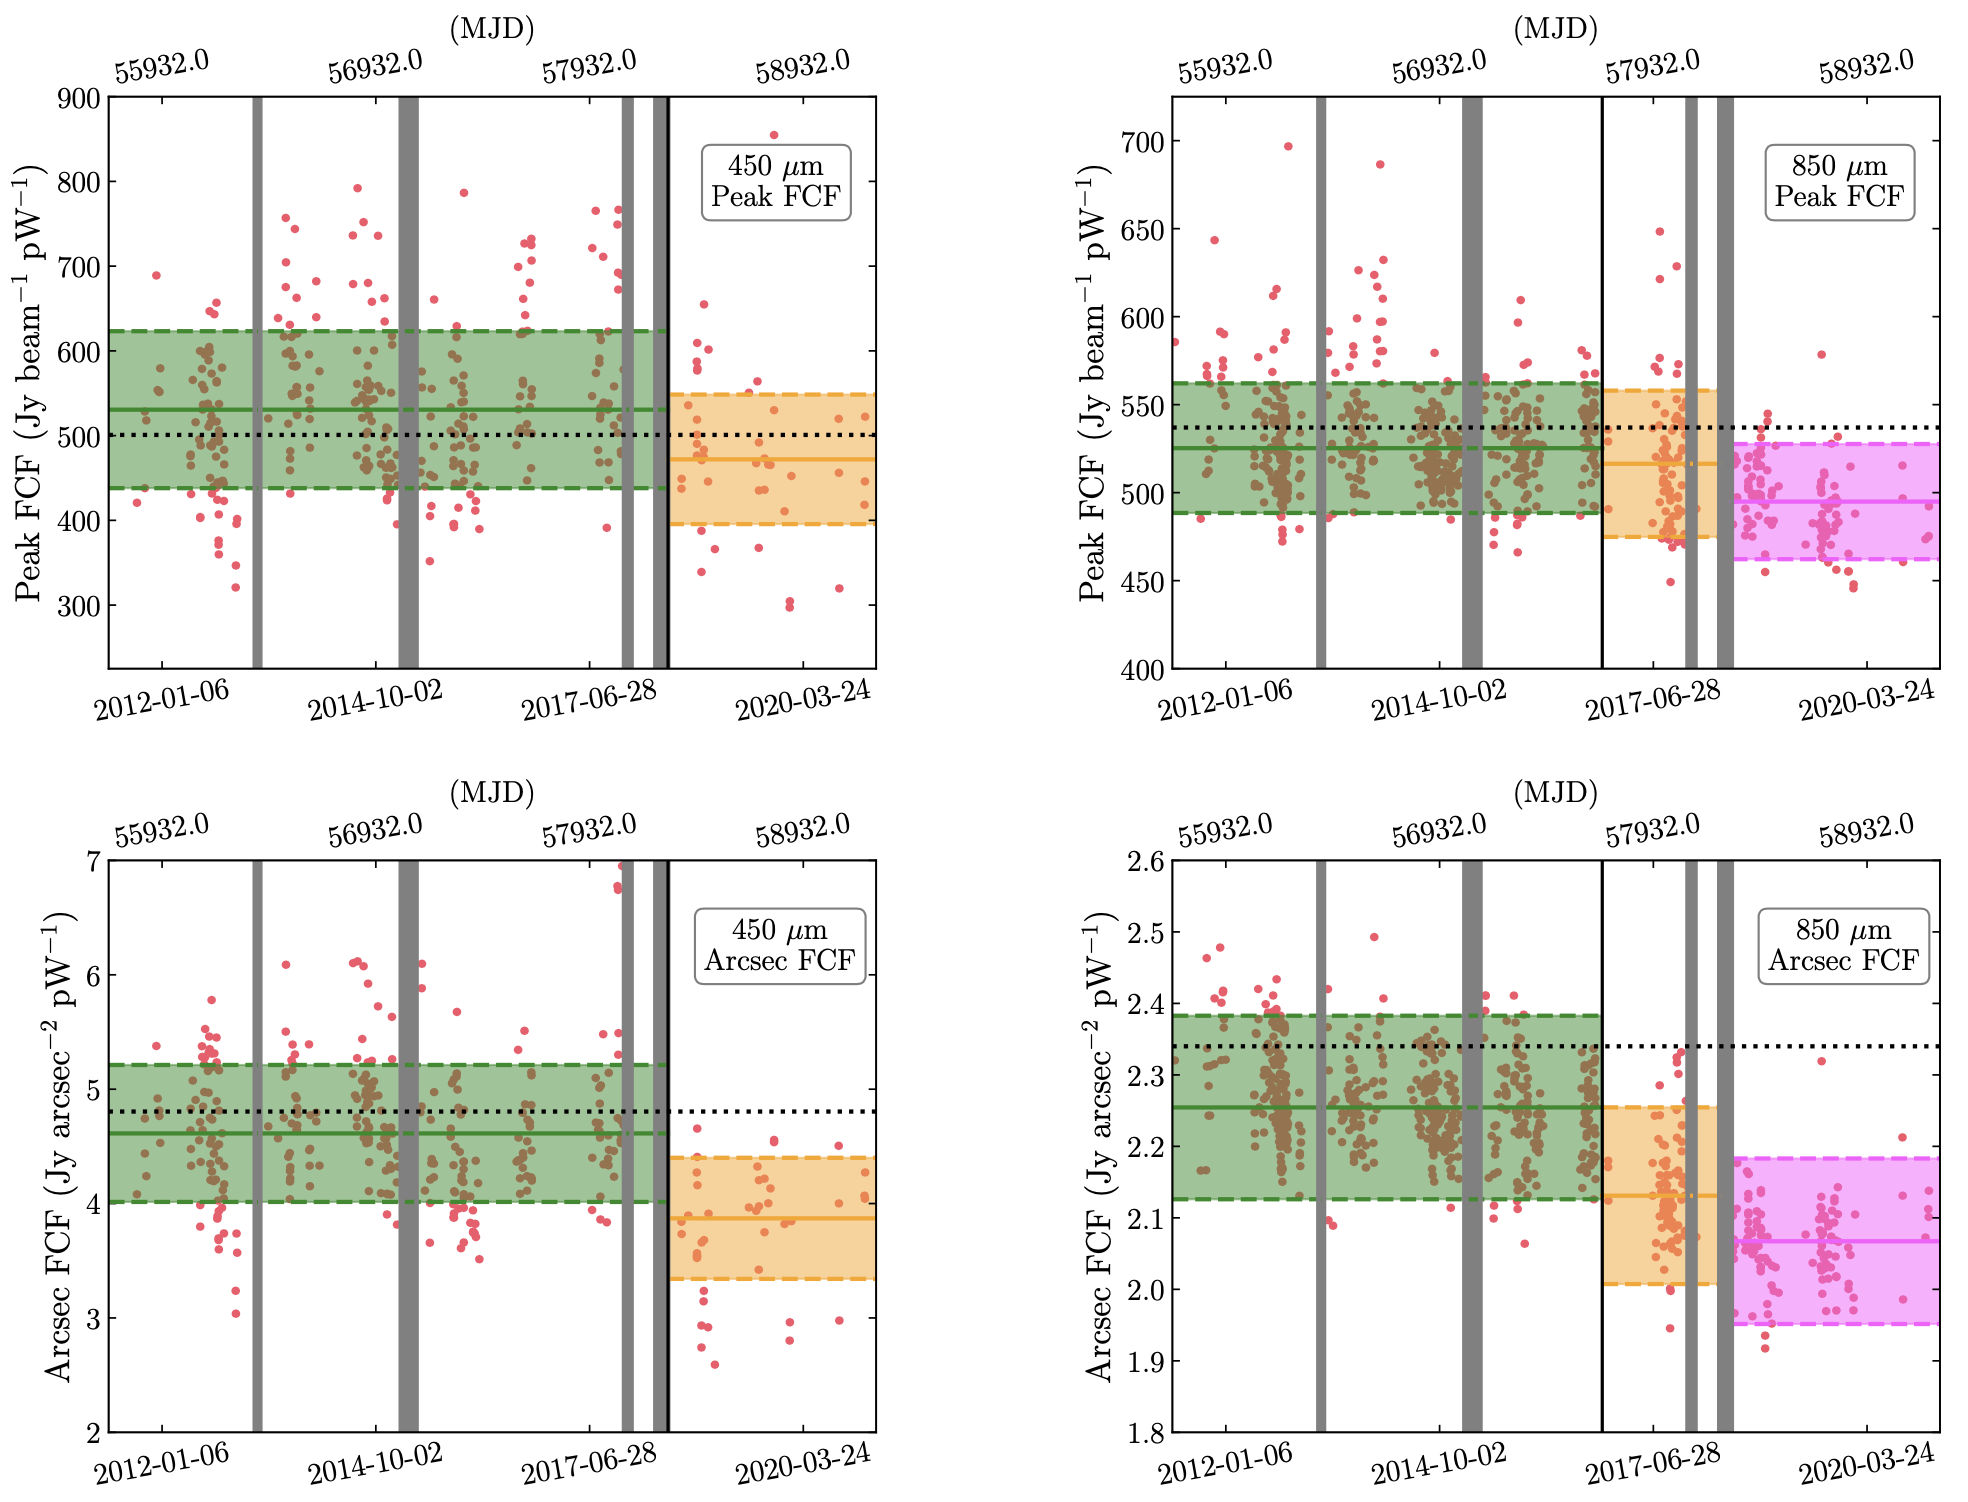
\includegraphics[width=0.9\linewidth]{sc21_FCFstep}
\caption[FCF step function]{From Mairs et al (2021)~\cite{mairs21}. FCFs derived using flux measurements of the primary calibrator Uranus during the stable part of the night (07:00-17:00 UTC) as a function of date. The gray shaded regions indicate epochs that are not included in the FCF determinations. The horizontal, shaded regions indicate the median FCF value over each span of time and the associated median absolute deviation added in quadrature with the 5\% uncertainty in the Uranus flux model. The black (dotted) lines indicate the original FCF value derived by Dempsey et al (2013)~\cite{dempsey12}, adjusted for the newly derived opacity relations, assuming the most common atmospheric transmissions during observations (see Figure 2). Left: Peak (Top) and Arcsecond (Bottom) FCFs derived at 450 microns. The solid, vertical line at the right edge of the latest gray region marks 2018 June 30 when the secondary mirror unit maintenance was completed. Data wherein the atmospheric transmission are less than 10\% are excluded. Right: Peak (Top) and Arcsecond (Bottom) FCFs derived at 850 microns. The solid, vertical line marks 2016 November, when the SCUBA-2 thermal filter stack was updated. Data wherein the atmospheric transmission are less than 25\% are excluded..}
\label{fig:FCFstep}
\end{figure}
\end{center}

\rule{1.0\textwidth}{2pt}

\textbf{Results from Dempsey et al. 2013 \cite{dempsey12}: employed by
default in Starlink Versions 2018A and previous.}\\
\begin{table}[h!]
\begin{center}
\begin{tabular}{|l|c|c|c|c|}
 \hline
 \multicolumn{1}{|c|}{Date} &
 \multicolumn{2}{c|}{FCF -- 450\,$\mu$m} &
 \multicolumn{2}{c|}{FCF -- 850\,$\mu$m} \\
\cline{2-5}
& Jy/pW/beam &Jy/pW/arcsec$^2$ & Jy/pW/beam &Jy/pW/arcsec$^2$ \\
 \hline
until 2012 January       & 383 & 4.9\hphantom{0} & 1080            & 5.0\hphantom{0} \\
2012 January--2012 July  & 606 & 6.06            & \hphantom{1}556 & 2.42 \\
2012 July onwards        & 491 & 4.71            & \hphantom{1}537 & 2.34 \\
\hline
\end{tabular}
\end{center}
\end{table}
\vspace{-2mm}
\begin{table}[h!]
\begin{center}
\begin{tabular}{|l|l|l|}
 \hline
 \multicolumn{1}{|c}{Date} & \multicolumn{2}{|c|}{Opacity Relationship}  \\ \cline{2-3}
                           & \multicolumn{1}{|c|}{450\,$\mu$m}    & \multicolumn{1}{|c|}{850\,$\mu$m} \\ \hline
until 2012 January         & 32 $\times$ ($\tau_{225}$ - 0.02)    & 5.2 $\times$ ($\tau_{225}$ - 0.013)  \\
2012 January--2012 July    & 26 $\times$ ($\tau_{225}$ - 0.01923) & 4.6 $\times$ ($\tau_{225}$ - 0.00435) \\
2012 July onwards          & 26 $\times$ ($\tau_{225}$ - 0.01196) & 4.6 $\times$ ($\tau_{225}$ - 0.00435) \\
\hline
\end{tabular}
\end{center}
\end{table}
